\documentclass{article}
\usepackage[T2A]{fontenc}
\usepackage[utf8]{inputenc}   
\usepackage[english, russian]{babel}

% Set page size and margins
% Replace `letterpaper' with`a4paper' for UK/EU standard size
\usepackage[a4paper,top=2cm,bottom=2cm,left=2cm,right=2cm,marginparwidth=1.75cm]{geometry}

\usepackage{amsmath}
\usepackage{graphicx}
\usepackage[colorlinks=true, allcolors=blue]{hyperref}
\usepackage{amsfonts}
\usepackage{amssymb}
% \usepackage[left=1cm,right=1cm,top=1cm,bottom=1cm]{geometry}
\usepackage{hyperref}
\usepackage{seqsplit}
\usepackage[dvipsnames]{xcolor}
\usepackage{enumitem}
\usepackage{algorithm}
\usepackage{algpseudocode}
\usepackage{algorithmicx}
\usepackage{mathalfa}
\usepackage{mathrsfs}
\usepackage{dsfont}
\usepackage{caption,subcaption}
\usepackage{wrapfig}
\usepackage[stable]{footmisc}
\usepackage{indentfirst}
\usepackage{rotating}
\usepackage{pdflscape}

\usepackage{MnSymbol,wasysym}


\begin{document}

\title{\textbf{Основные алгоритмы. Домашняя работа 6 неделя}}


\author{Зайнуллин Амир}
\maketitle

\section*{Задача №1}

Нарисуем доску $n \cdot n$. Позиция, из которой нельзя сделать ход (то есть нельзя сдвинуть по горизонтали влево и по вертикали вниз) является левая нижняя клетка. То есть является $P$ позицией.

\begin{table}[!ht]
    \centering
    \begin{tabular}{|c|c|c|c|c|c|c|c|}
    \hline
        ~ & ~ & ~ & ~ & ~ & ~ & ~ & ~ \\ \hline
        ~ & ~ & ~ & ~ & ~ & ~ & ~ & ~ \\ \hline
        ~ & ~ & ~ & ~ & ~ & ~ & ~ & ~ \\ \hline
        ~ & ~ & ~ & ~ & ~ & ~ & ~ & ~ \\ \hline
        ~ & ~ & ~ & ~ & ~ & ~ & ~ & ~ \\ \hline
        ~ & ~ & ~ & ~ & ~ & ~ & ~ & ~ \\ \hline
        ~ & ~ & ~ & ~ & ~ & ~ & ~ & ~ \\ \hline
        P & ~ & ~ & ~ & ~ & ~ & ~ & ~ \\ \hline
    \end{tabular}
\end{table}

На семинаре и на лекции объясняли, что все клетки, у которых существует последователь $P$, является $N$ позицией. Для всей левой вертикали и нижней горизонтали (кроме нижней левой клетки) существует последователь $P$ (нижняя левая клетка). Значит вся левая вертикаль и нижняя горизонталь (кроме нижней левой клетки) является $N$ позицией.

\begin{table}[!ht]
    \centering
    \begin{tabular}{|c|c|c|c|c|c|c|c|}
    \hline
        N & ~ & ~ & ~ & ~ & ~ & ~ & ~ \\ \hline
        N & ~ & ~ & ~ & ~ & ~ & ~ & ~ \\ \hline
        N & ~ & ~ & ~ & ~ & ~ & ~ & ~ \\ \hline
        N & ~ & ~ & ~ & ~ & ~ & ~ & ~ \\ \hline
        N & ~ & ~ & ~ & ~ & ~ & ~ & ~ \\ \hline
        N & ~ & ~ & ~ & ~ & ~ & ~ & ~ \\ \hline
        N & $*$ & ~ & ~ & ~ & ~ & ~ & ~ \\ \hline
        P & N & N & N & N & N & N & N \\ \hline
    \end{tabular}
\end{table}

Также показывали, что те клетки, у который любой последователь является $N$ позицией, является $P$ позицией. Рассмотрим клетку $*$. У нее существует два последователя, это нижняя и левая клетка. Так как они являются $N$ позицией, то $*$ является $P$ позицией.

\begin{table}[!ht]
    \centering
    \begin{tabular}{|c|c|c|c|c|c|c|c|}
    \hline
        N & ~ & ~ & ~ & ~ & ~ & ~ & ~ \\ \hline
        N & ~ & ~ & ~ & ~ & ~ & ~ & ~ \\ \hline
        N & ~ & ~ & ~ & ~ & ~ & ~ & ~ \\ \hline
        N & ~ & ~ & ~ & ~ & ~ & ~ & ~ \\ \hline
        N & ~ & ~ & ~ & ~ & ~ & ~ & ~ \\ \hline
        N & ~ & ~ & ~ & ~ & ~ & ~ & ~ \\ \hline
        N & P & ~ & ~ & ~ & ~ & ~ & ~ \\ \hline
        P & N & N & N & N & N & N & N \\ \hline
    \end{tabular}
\end{table}

\newpage

Далее рассуждая аналогичным образом, сможем получить такую таблицу.

\begin{table}[!ht]
    \centering
    \begin{tabular}{|c|c|c|c|c|c|c|c|}
    \hline
        N & N & N & N & N & N & N & P \\ \hline
        N & N & N & N & N & N & P & N \\ \hline
        N & N & N & N & N & P & N & N \\ \hline
        N & N & N & N & P & N & N & N \\ \hline
        N & N & N & P & N & N & N & N \\ \hline
        N & N & P & N & N & N & N & N \\ \hline
        N & P & N & N & N & N & N & N \\ \hline
        P & N & N & N & N & N & N & N \\ \hline
    \end{tabular}
\end{table}

Видно, что все $P$ позиции это диагональ из левого нижнего угла в правый верхний. Что и требовалось доказать. 

\section*{Задача №2}

Пусть первый кладет каждый раз по 2 монеты. Построим граф ходов. Зеленые ребра - ходы первого, красные - ходы второго. Вершина с 20 монетами является $P$ позицией. Пометим остальные вершины графа согласно правилам, которые были описаны в прошлом задании.

\begin{figure}[!ht]
    \center{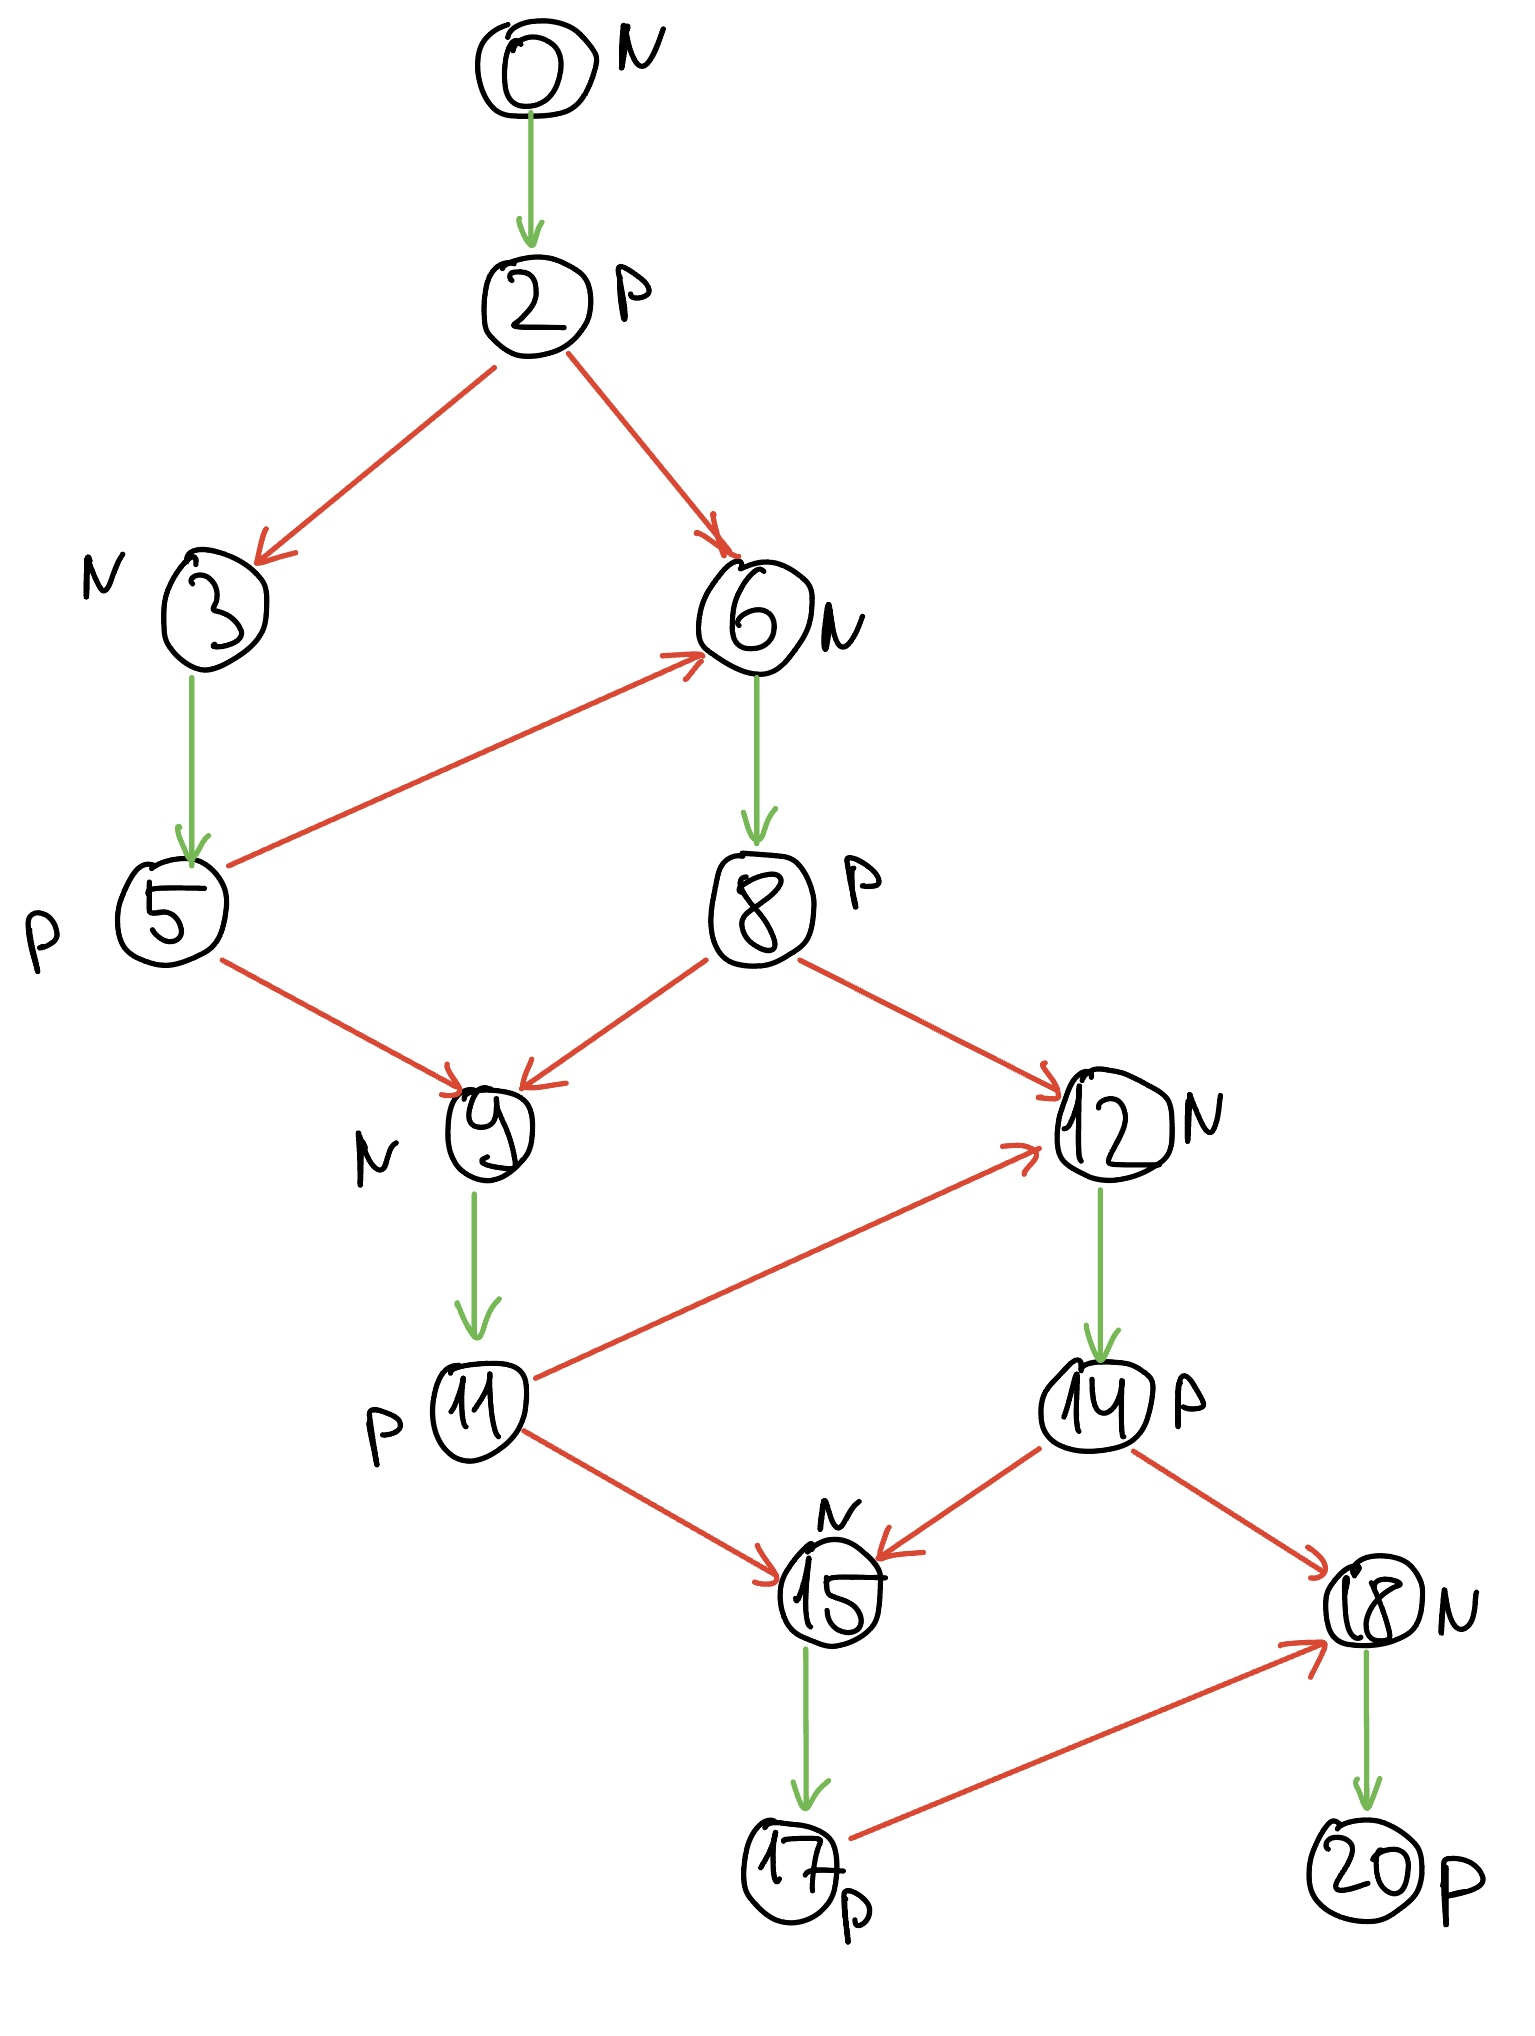
\includegraphics[width=0.7\textwidth]{img1.png}}
\end{figure}

\newpage

Видно, что данная стратегия первого является выигрышной. Действительно, прибавляя к монетнице по 2 монеты, при любом ходе второго, который может класть только 1 или 4 монеты, после хода второго количество монет в монетнице будет делиться на 3. Также это видно из графа, все красные ребра ведут в вершины с количеством монет которое делится на 3. После хода второго никак не получится 20 монет в монетнице, так как 20 не делится на три.

\section*{Задача №3}

Пометим все листья как плохие или хорошие. Хорошими будут листья белого цвета. Плохими будут листья черного цвета. Если мы попадем на вершину красного цвета - мы проиграли. Если попали в зеленого цвета, то выиграли. Сейчас наш уровень - $4^n$ листьев. Далее будем подниматься на уровень выше. Рассмотрим каждую вершину с этого уровня. Переход с этой вершины на уровень ниже - это ход преподавателя. Если хотя бы один сын плохой, то вершина тоже будет плохой (потому что преподаватель может сходить в плохую и выиграть). Если плохого сына нет, то вершина будет хорошей. Теперь поднимемся еще на уровень выше. Теперь переход с этого уровня на ниже соответствует нашему ходу. Если есть хотя бы один хороший сын, то вершина будет хорошей. (потому что мы сходим в хорошую). Если хорошего сына нет, то вершина плохая. Далее будем подниматься согласно тому, как было описано до этого (опять ход преподавателя, потом наш и т.д.)

Пример данного графа (зеленый - хороший, красный - плохой). В данном случае выиграем мы (студент), так как верхняя вершина зеленая.

\begin{figure}[!ht]
    \center{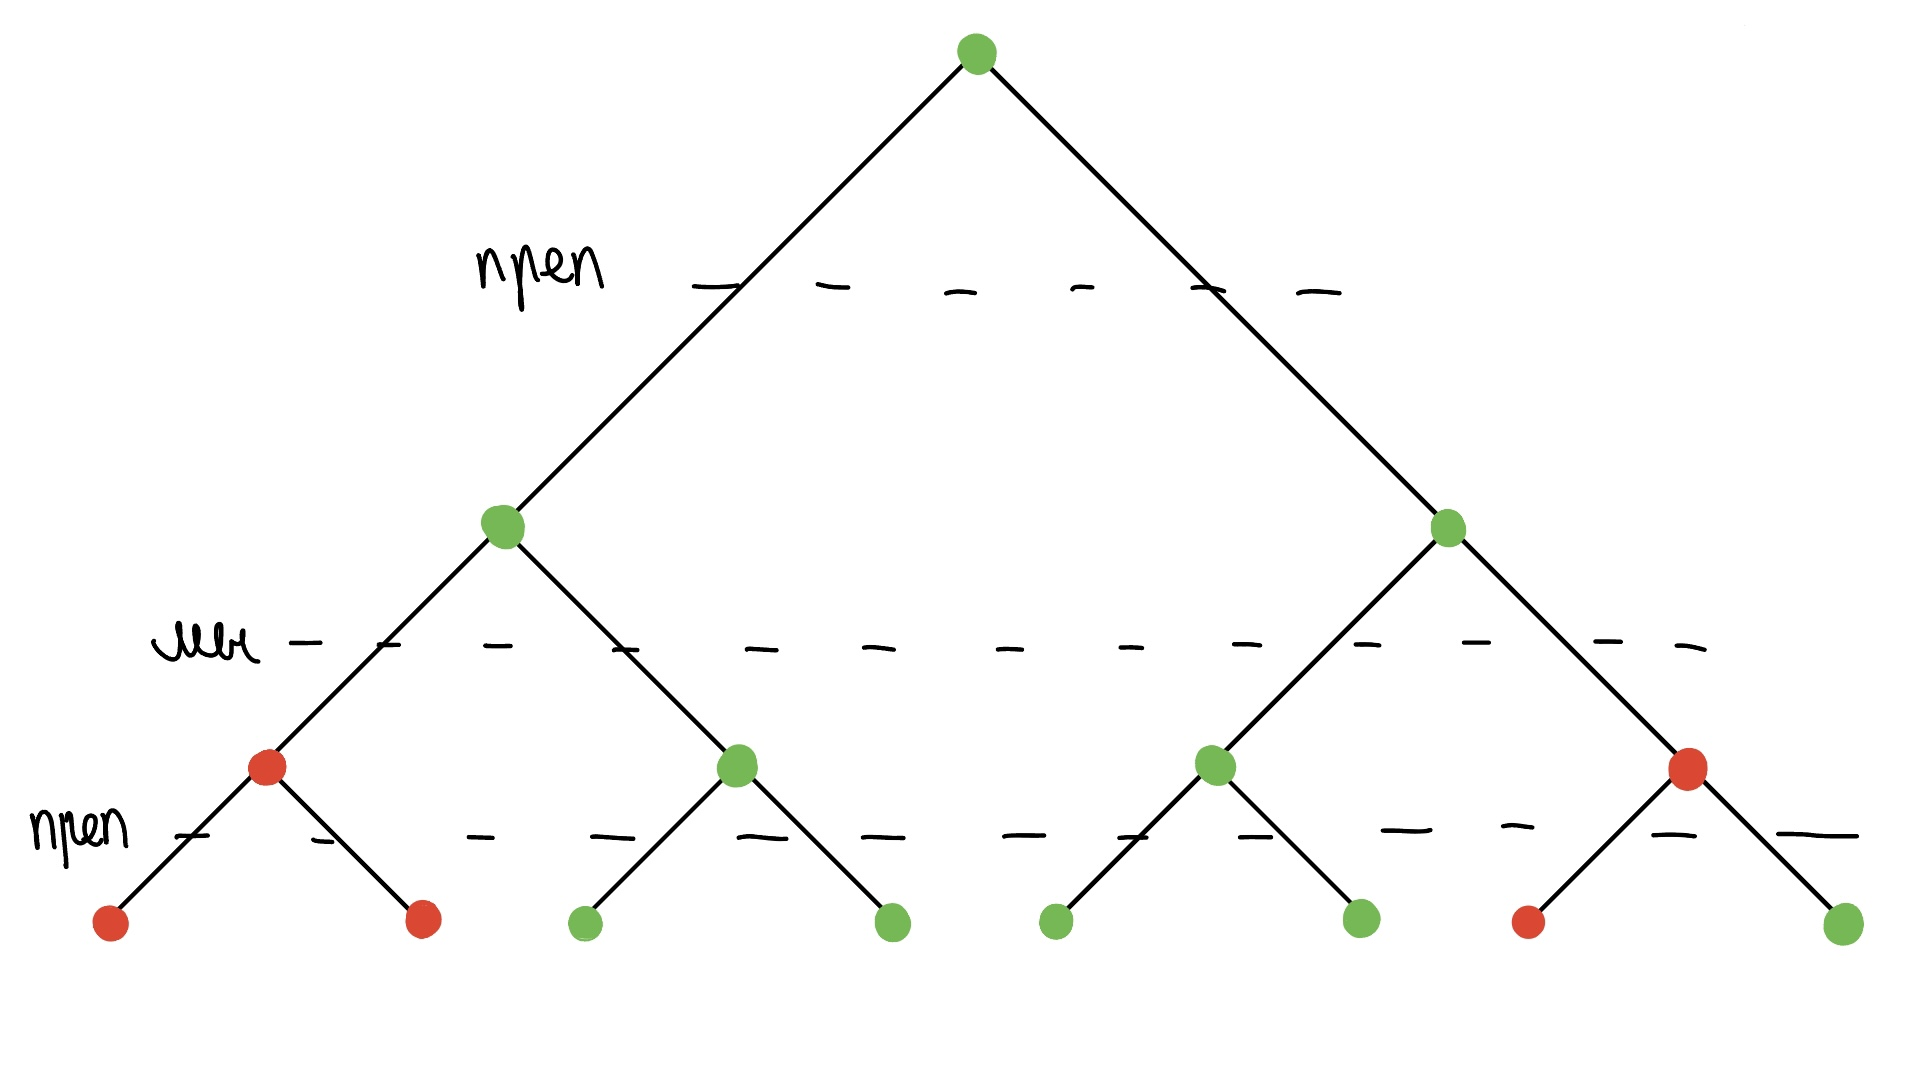
\includegraphics[width=0.8\textwidth]{img2.jpg}}
\end{figure}

\end{document}